%!TEX TS-program = xelatex
% Much of lab manual was taken from Jonathan Peelle's lab manual. 
% See original source here: https://github.com/jpeelle/peellelab_manual/

\documentclass[letterpaper,12pt,oneside]{memoir}
\usepackage{color}
\usepackage[pdftitle={Smith Lab Manual}, pdfauthor={David V. Smith}, colorlinks=true, urlcolor=blue]{hyperref}
\usepackage{multicol}
\usepackage{array,ragged2e}
\usepackage{fontspec,xunicode}
\defaultfontfeatures{Mapping=tex-text}
\setromanfont{Cambria}
\definecolor{shadecolor}{gray}{0.9}
\setsecnumdepth{section}
\maxtocdepth{subsection}
\usepackage{multicol}
\usepackage{enumitem}

\chapterstyle{article}



%\pretitle{\huge\sffamily}
%\posttitle{\vskip 0.5em}
% \preauthor{\begin{flushleft}}
%\postauthor{\end{flushleft}}
%\predate{\begin{flushleft}}
 %\postdate{\end{flushleft}}

\setlength{\droptitle}{1in}

\checkandfixthelayout	% for memoir class

\begin{document}

\title{Smith Lab Manual}
\author{David V. Smith\\Department of Psychology\\Temple University}
\date{\today}

%\href{https://sites.google.com/a/temple.edu/dvs-lab/SmithLab\_manual.pdf}{Link to Lab Manual}

\maketitle

\pagestyle{titlingpage}


\cleardoublepage
\frontmatter
\tableofcontents
\cleardoublepage

\mainmatter

\pagestyle{headings}

%%%%%%%%%%%%%%%%%%%%%
\chapter{Introduction}

My overarching goal is to foster an environment of scientific excellence and personal development for all lab members. We should continually strive to learn and improve---and we should also try to have fun doing great science. This Lab Manual\footnote{Much of this document is derived from or copied directly from Dr. Jonathan Peelle's excellent \href{https://github.com/jpeelle/peellelab\_manual/}{Lab Manual}.} is meant to be the first resource for the lab as we seek to achieve these goals. You can also find the lab elsewhere:

\begin{itemize}[noitemsep]
\item Website: \url{https://sites.temple.edu/neuroeconlab/}
\item GitHub: \url{https://github.com/DVS-Lab}
\item Twitter: \url{https://twitter.com/DVSneuro}
\item Mendeley: \url{https://www.mendeley.com/community/smith-lab-meetings/}
\item OSF: \url{https://osf.io/5zq6h/}
\end{itemize}

\noindent There are also a couple of sites accessible only by lab members:

\begin{itemize}[noitemsep]
\item Wiki: \url{https://smithlabwiki.cla.temple.edu}
\item Trello: \url{https://trello.com/neuroeconomicslaboratory}
\item Slack: \url{https://neuroeconomicslab.slack.com}
\end{itemize}

In general, firm policies are in the lab manual, whereas ways of implementing those policies (i.e., getting stuff done) should be on the Wiki so that they can be updated by anyone in the lab. Trello organizes tasks that need to be done (and relevant discussions, with the help of Slack) for specific projects, rather than general principles. Any information that is potentially private or sensitive should go in a protected location. (You can read more about various lab resources in \Sref{sec:communicationInLab} on \pref{sec:communicationInLab}.)

The \LaTeX\ source for the lab manual is available on \href{https://github.com/dvsneuro/smithlab_manual}{GitHub}.

\begin{shaded}
\noindent I assume the Lab Manual and Wiki are accurate and clear. This means that you should follow all of the policies and protocols contained in the manual and Wiki. If you notice something that seems to be wrong (or missing), please let me know (for the lab manual) or change it yourself (for the wiki). If there is something in the lab manual or wiki that you notice people aren't doing, please bring this up at lab meeting, or to me, privately---don't assume this is okay (it's not).
\end{shaded}


%%%%%%%%%%%%%%%%%%%%%
\chapter{General} % About the lab

\section{Funding}

Grant funding supplies the much of resources needed to conduct our research, including salary for personnel, RA-ships for PhD students, equipment, subject payments, and so on. It is important that we run the lab in a way that shows we use our research funding carefully. 

Our current grant funding includes:

\begin{itemize}

\item Targeted Small Grant Award from OVPR at Temple University titled ``Modulating Individual Differences in Reward Sensitivity with Transcranial Current Stimulation" (active: 2018-01-01 to 2019-12-31). This project examines how transcranial current stimulation impacts reward processing and decision making.
\item R21-MH113917 from NIMH titled ``Remote Modulation of Reward Circuits with Noninvasive Brain Stimulation" (active: 2017-07-05 to 2019-04-30). This project is focused on how transcranial alternating current stimulation modulates neural and behavioral responses to reward. 
\item Pilot Grant from SRNDNA titled ``Social Reward and Aging: Identifying the Neural Underpinnings of Peer Influences" (active: 2017-10-01 to 2018-12-31). This project is focused on how the relationship between trust and social closeness changes across the lifespan. 

\end{itemize}

Funding from NIH means that work in the lab is supported by the taxpaying public---and we should strive to produce products that show we are using the money wisely. Startup funds should be viewed similarly. 

\section{Local Collaborators}
Our local collaborators (i.e., those at Temple) are in involved in active or pending grants. Although the work on some of these projects has not yet begun, I include pending projects that are likely to materialize in some form or another soon (e.g., funded grant or additional pilot data collection).

\begin{multicols}{2}
\begin{itemize}[noitemsep,nolistsep]
\item Lauren Alloy
\item Jason Chein
\item Eunice Chen
\item Tania Giovanetti
\item Johanna Jarcho
\item Vishnu (Deepu) Murty
\item Ingrid Olson
\item Crystal Reeck
\item Jamie Reilly
\item Vinod Venkatraman
\end{itemize}
\end{multicols}

\section{Other Collaborators}

We also have a number of collaborators who have a home outside of Temple. These individuals are also involved in active/pending grants or manuscripts that are in preparation. 

\begin{itemize}[noitemsep,nolistsep]
\item Pamela Butler (Nathan Kline Institute and New York University)
\item John Clithero (University of Oregon)
\item Mauricio Delgado (Rutgers University --- Newark)
\item Dominic Fareri (Adelphi University)
\item Bart Krekelberg (Rutgers University --- Newark)
\item Chris Rorden (University of South Carolina) 
\end{itemize}



%%%%%%%%%%%%%%%%%%%%%
\chapter{Being in the lab}

\section{Everyone}

\subsection{Big picture}

We expect each other to:

\begin{itemize}
\item Push the envelope of scientific discovery and personal excellence. 
\item Do work we are proud of individually and as a group.
\item Double-check our work, and be at least a little obsessive.
\item Be supportive---we're all in this together.
\item Be independent when possible, ask for help when necessary.
\item Communicate honestly, even when it's difficult.
\item \textbf{Share your knowledge}. Mentorship takes many forms, but frequently involves looking out for those more junior.
\item Be engaged in the scientific community. Everyone should be able to \textit{get} help and \textit{give} help on mailing lists and discussion boards, such as \href{https://neurostars.org}{NeuroStars}.
\item Work towards proficiency in Unix, BASH, Matlab, R, and Python (bonus points for Javascript and \LaTeX).
\item Be patient with everyone, including with your PI (he will forget things you just talked about and be busier than he would like).
\item Advocate for our own needs, including personal and career goals.
\item Respect each other's strengths, weaknesses, differences, and beliefs.
\end{itemize}

We should also expect everyone to have a professional and accurate online presence. If you have an online profile somewhere (e.g., LinkedIn, NeuroStars, ResearchGate, Twitter, Google Scholar, etc.), keep it up to date and professional. Remember, we all represent the lab and the lab represents us. Let's make sure we have an excellent online presence.


\subsection{Small picture}

We're sharing a relatively small space, so please be thoughtful of others, including (but not limited to):

\begin{itemize}
\item With few exceptions, \textbf{do not come to the lab if you are sick}. It's better to keep everyone healthy. If you are sick, email the lab manager or me to let me know you won't be coming in, and update your lab calendar to reflect the change.
\item Do not leave food, drinks, or crumbs out in the lab. Please put food trash in another trash can (not in the lab), especially late in the day or on Friday (so that food doesn't stay in the lab overnight).
\item Avoid wearing strong perfumes/colognes/etc.\ in the lab (for the sake of your coworkers and our participants).
\item Keep the lab neat---especially in the entryway area. Items left unattended may be cleaned, reclaimed, or recycled.
\item Turn off or minimize notifications on your devices. Although it is important to be available for emergencies, you might find yourself sifting through countless notifications and attending to nonstop alerts if the notification settings on your devices aren't constrained.
\end{itemize}


\section{The Boss}

You can expect me to:

\begin{itemize}
\item Have a vision of where the lab is going.
\item Care about your happiness.
\item Obtain the funding to support the science, and the people, in the lab.
\item Support you in your career development, including writing letters of recommendation, introductions to other scientists, conference travel, and promoting your work as often as possible.
\item Support you in your personal growth by giving you flexibility in working hours and environment, and encouraging you to do things other than science.
\item Make the time to meet with you regularly, read through your manuscripts, and talk about science.
\item Obsess over running the right analyses, writing clearly, and making beautiful figures.
\end{itemize}


%\section{Postdocs}

%I expect postdocs to move towards being more PI-like, including giving talks, writing grants, and cultivating an independent research program (while still supporting the lab's research). And, to have (or acquire) the technical and open science skills listed for PhD students, below.

%If you are supported by a specific grant, which will usually be the case, [you shouldn't expect to stay past that grant?]

%Postdoc salaries generally follow NIH guidelines (regardless of the source of funding).

\section{PhD students}

I expect PhD students to:

\begin{itemize}
\item Know the literature related to their topic like the back of their hand. For more information about staying on top of the literature, see \Sref{sec:literature} on \pref{sec:literature}.
\item Be \textbf{excited} about the research questions they are asking and \textbf{eager} to find the answers. (If I am more eager to know the answer(s) to your research questions, we need to rethink your research questions.)
\item Seek out and apply for fellowships and awards, including external and internal travel awards and training workshops.
\item Realize there are times for pulling all nighters, and times for leaving early to go to the park and enjoy the sunshine.
\end{itemize}

By the time you're done, you will have developed a full spectrum of skills needed to become a great scientist---from hard skills (e.g., technical and analytical) to soft skills (e.g., communication and teamwork)\footnote{\url{https://loop.nigms.nih.gov/2015/11/catalyzing-the-modernization-of-graduate-education/}}. For example, you will develop a program of research that speaks to a significant problem or open question in the field. In service of this, you will conduct carefully-executed experiments and communicate your results clearly, both in written and verbal formats. 

In addition, you will also know how to do statistics and plots in R, Matlab, and/or Python, share your work with me using GitHub/OSF, Rmarkdown, and/or Jupyter Notebooks, write Matlab and BASH scripts for data analyses, know enough Python to navigate presentation in PsychoPy and do simple scripting, and make figures and posters using Adobe Illustrator or a similar vector-based graphics program (e.g., Inkscape). You will also preregister your experiments when appropriate (which it almost certainly will be) and share your data and analysis scripts publicly. These skills are essential ingredients for success in cognitive neuroscience and industry (for more information, see \Sref{sec:coding} on \pref{sec:coding}).

The learning curve can be a little steep on all of these learning objectives---but it's well worth it. If these objectives aren't compatible with your goals or interests, then my lab is probably not a good fit for you!



\section{Employees}

I expect paid employees, whether full-time or part-time, to use their time efficiently to support the projects to which they are assigned. Paid employees will typically have the most interaction with other staff, and with research participants, and in these contexts especially should be a model of professionalism.

\subsection{Hours}
Work hours in the lab are 8:00--5:00 (or 9:00--6:00), with 60 minutes for lunch by default. If you are testing participants outside of this time, we will adjust accordingly for those weeks. You are responsible for keeping your hours at the agreed amount (8 hours per day, 40 hours per week for full-time employees). To maintain full-time benefits eligibility your hours cannot drop (much) below 35; if on a given week you work substantially less than 30 hours, vacation time may be used to make up the difference \href{http://www.temple.edu/hr/departments/employeerelations/documents/Employee_Manual_Feb_2016.pdf}{(per HR policy)}.

Time off should be requested at least 2 weeks in advance, via email. Once approved (via email) please add to the lab calendar. You are responsible for making sure you have sufficient vacation hours to cover any time off; otherwise, you will not be paid.

Sick time should also be requested over email. Per HR policy, full-time employees are earned sick days at the rate of 1 day/month up to 10 days up (these sick days carry over to the next fiscal year).

(Note that graduate students, postdocs, and staff scientists are generally given more flexibility in their hours, provided they make sufficient progress on their projects. This flexibility does not generally extend to other paid positions because we need to maintain a consistent lab presence for scheduling, supporting undergrads, interacting with other staff, and so on.)

\begin{shaded}
\noindent Even if you speak with me in person, it is important to document these requests (and my approval) over email so that we have a record. It is your responsibility to make sure this happens.
\end{shaded}

\subsection{Timesheets}

\begin{itemize}
\item Hours entered on your timesheet should reflect hours actually at work.
\item Monitor your time carefully and do not forgot to clock in/out in the lobby. If you forget to clock out or your hours appear anomalous, it creates extra work for someone else to fix. 
\item Clock out for breaks 60 minutes or longer (this is your default lunch, unless we've changed it in Kronos to 30 minutes).
\item If you're not using the clock-in/clock-out system in the lobby (e.g., testing off campus), submit your timesheet before the due date.
\end{itemize}


\subsection{Employee resources}

There are many resources and benefits available through \href{https://www.temple.edu/faculty-and-staff/working-temple/human-resources}{human resources}. These policies are spelled out to some degree on the HR website and in the \href{http://www.temple.edu/hr/departments/employeerelations/documents/Employee_Manual_Feb_2016.pdf}{Employee Manual}, and I can also put you in touch with people in the department or HR who can offer guidance.

\section{Masters students}
I expect masters students will be organized and independent, and manage their research time and classroom responsibilities so that they complete a project by the end of their second year, which requires being somewhat strategic in the topic we pick. The written report is typically due at the end of April, with an oral presentation in early May. In some cases, I will encourage you to pursue a \href{https://cos.io/rr/}{Registered Report}, which focuses your time and energy on reviewing the literature, developing your questions and hypotheses, and designing the experiment to evaluate your hypotheses. You should aim to have an ``in principle acceptance" of your registered report by the middle of the Fall semester of your second year so that you can complete some of the data collection and analyses before the end of your program.

If a Registered Report is not appropriate for your project, timeline, or goals (e.g., you want to spend more time on data collection or analysis), then we need to adjust our plan and collect data sooner. To collect a reasonable amount of data, it is almost always necessary to start collecting data during the Fall semester, which is challenging because of classroom responsibilities. Don't say I didn't warn you!

At the outset of your masters project, please create a Trello board and make a check list with planned due dates (e.g., see Table \ref{table:deadlines}), and keep this updated throughout the year.

\section{Undergraduate students}

\subsection{Honors students}

Students who have already demonstrated themselves to be careful and independent workers for a minimum of 3 months may apply to do an honors project in the lab. The overall project should be discussed in the Spring for completion the following year. Due dates and requirements differ across programs; check with your individual program for application requirements. I expect that we will start working on this over the summer before the project year, whether that involves you working in the lab over the summer, or working from home.

Because honors projects necessarily rely on lab resources, they need to fit within the overall scope of lab research. I work with the graduate students and postdocs to create list of possible honors projects to choose from which fit within our ongoing research which we can use as a starting point for our discussions.

The paperwork requirements differ by program. It is your responsibility to check what the requirements are in your program and department, and make sure to get your project submitted by the deadline (which might be the semester before your senior year).

At the outset of your honors project, please make a check list with planned due dates (e.g., see Table \ref{table:deadlines}), and keep this updated throughout the year.

% table describing deadlines for student projects
\begin{table}
\centering
\caption{Deadlines for short-term research projects}
\begin{tabular}{lcc}
\toprule
& Senior honors & Masters\\
\midrule
Topic picked& \multicolumn{2}{c}{Spring of prior year}\\
Stimulus materials finalized& \multicolumn{2}{c}{September 1}\\
IRB approval finalized& \multicolumn{2}{c}{September 15}\\
Data collection begun& \multicolumn{2}{c}{October 1}\\
15 minute lab talk on background& \multicolumn{2}{c}{Fall semester}\\
Draft of introduction and methods& \multicolumn{2}{c}{December 20}\\
Complete written draft& March 1& April 1\\
Practice talk& April 1 & April 15\\
Final written draft& End of April & End of April\\
Oral presentation& After Spring break & Early May\\
\bottomrule
\end{tabular}
\label{table:deadlines}
\end{table}

\subsection{Independent study students}
Undergraduate students in the lab during the year should enroll in an independent study section to receive credit for time in the lab.

Independent study students should plan on producing an annotated bibliography of 5--10 articles on their selected topic, and making a 15-minute presentation at lab meeting sometime during the semester. (Depending on what department you are enrolled through, you may have additional requirements.)



\subsection{All undergraduates}

I expect undergraduates to be utterly reliable and willing to help with whatever projects need it. At a bare minimum, reliability includes showing up on time, maintaining your hours on the lab calendar, and making sure that all of your work is accurate (double-check everything). If you find yourself without a specific project:

\begin{itemize}
\item Ask around to see if you can help with anything.
\item Look on the wiki under ``Essential lab skills'' and spend some time learning something new.
\item Look on Trello for either a wiki page that needs creating/updating, or other miscellaneous lab tasks that need to be done.
\end{itemize}

There is enough to do that you should not be bored!

Your first semester in the lab is an opportunity to see whether continuing in the lab is a good fit; after your first semester we will meet and discuss whether you will continue.

\section{University policies}

\subsection{Employee guidelines}
Important guidance on benefits and policies (including time off policies and the Employee Handbook) are available on the \href{https://www.temple.edu/faculty-and-staff/working-temple/human-resources}{human resources website}. It is important that these policies are followed at all times. You are responsible for reviewing the policies and benefits; human resources is a good resource and they can help you if you have any questions.

\subsection{Sexual harassment}
University policy requires that if any faculty member (such as me) becomes aware of sexual harassment or abuse involving students or employees we must report it to the Title IX Sexual Harassment Response Coordinator. Counselors and other medical professionals on campus who discuss these issues in their professional capacity can keep patient confidentiality.


% http://www.temple.edu/hr/departments/employeerelations/documents/Employee_Manual_Feb_2016.pdf

%%%%%%%%%%%%%%%%%%%%%
\chapter{Communication}
\section{Communication within the lab}
\label{sec:communicationInLab}

I am usually busier than I'd like to be, and as a result have less time for talking to folks than I'd like. However, you (lab members) are one of the most important parts of my job, and I need your help to stay organized and involved in the things I need to be involved in. Some general rules of thumb are:

\begin{enumerate}
\item Be proactive---tell me what you need. This includes coming to knock on my door even if it seems like you are interrupting, emailing me to set up a time to meet, or catching me before or after lab meeting. In all likelihood I will not check in with you as often as I'd like, so it is up to you to make sure nothing falls through the cracks.

\item Write things down and remind me what we've talked about. I would love to remember everything we decided when we met last week, but this doesn't always happen. Don't hesitate to bring me up to speed when we meet. Even if I already remember what we are talking about, a couple of introductory topic sentences will help get me in the right frame of mind. Be sure to write down everything in your lab notebook and Trello!

\item Read all of the lab documentation: this lab manual, the lab wiki, and Trello. You are responsible for knowing what is in each of these places, following the rules and guidelines we have set up, and notifying someone if you find incorrect or unclear information (or if you have questions).

\item I can be the most helpful to everyone if you are a little bit strategic in what you ask me. Please check the lab wiki, other people in the lab, and a Google search before shooting me off a question (see Figure~\ref{fig:decisiontree}).

\end{enumerate}


\begin{figure}
\label{fig:decisiontree}
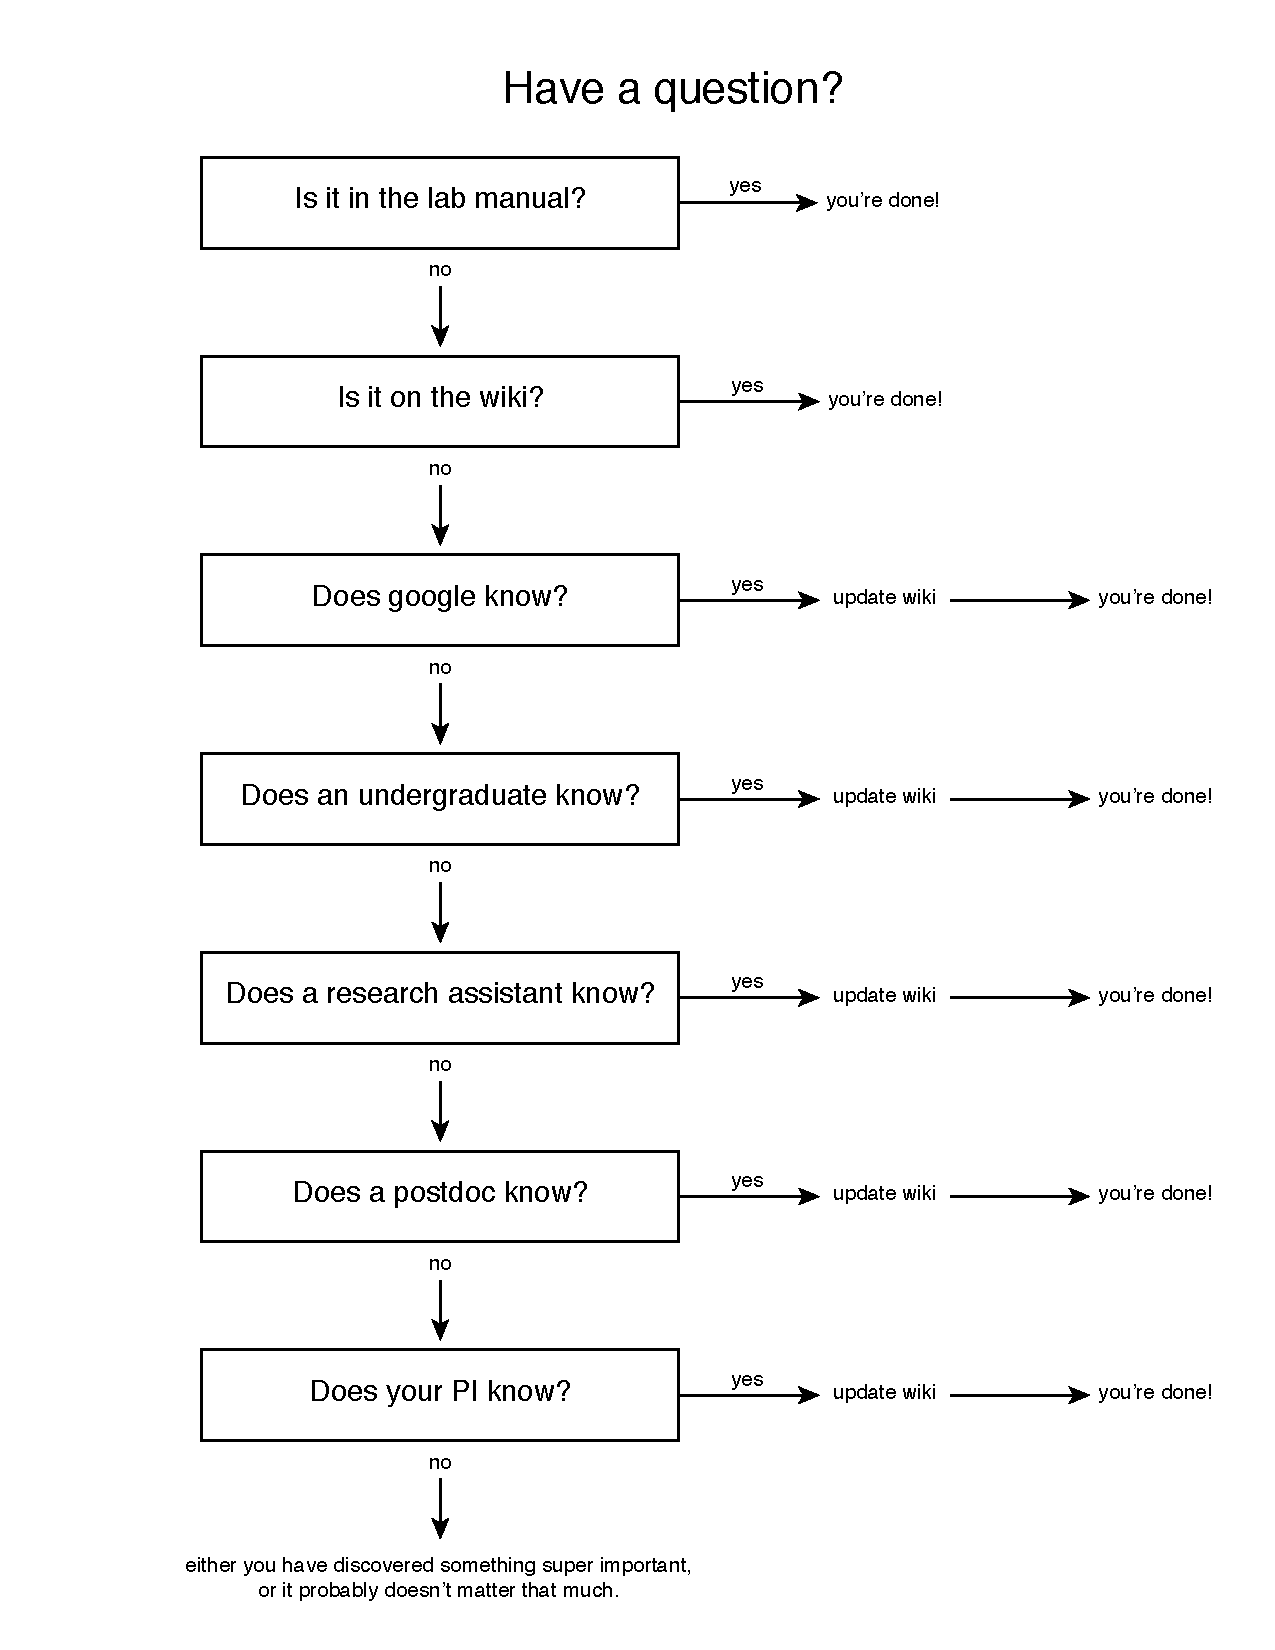
\includegraphics[width=\textwidth]{figures/lab_decision_tree.pdf}
\caption{Lab decision tree. Answers to all your questions should be in the lab wiki!}
\end{figure}

\subsection{My door}
Metaphorically my door is always open, but sometimes my door is, physically, closed (or perhaps slightly cracked open). If this is the case:

\begin{itemize}
\item If we have a meeting scheduled, then please knock. Hopefully I am around.

\item If we don't have a meeting scheduled, a closed door generally means I am trying to do some writing and should not be interrupted. Of course, if it's an emergency, please knock anyway. Otherwise, please send me a Slack direct message or try another time.
\end{itemize}

\subsection{Lab meeting}
We meet once each week to talk about science together, and to make sure we have a chance to touch base on administrative and practical issues. There may even be a snack. Regular attendance and participation is expected (unless you have a class or clinical responsibilities during that time).

Our lab meetings are 1.5 hours. During that time, we normally have two presenters: 1) one person leads a journal club on a recent empirical paper that is relevant to the lab; and 2) another person presents their work, a project proposal, a tutorial, or a general-interest topic that is worth a group discussion. Example general-interest topics might include a recent influential review paper, responsible conduct of research, professional development, or innovative research practices. Each person is allowed a maximum of 45 minutes. 


\subsection{Trello and Slack}
Trello and Slack are the main tools for lab communication and are preferred to email in almost every situation. Please help me by keeping these up to date! A few thoughts and tips:

\begin{itemize}
\item Create a Trello board and Slack channel for each of your projects.

\item Avoid direct messages for project-related discussions or questions. Instead, create and use a specific Slack channel for your project. You should be comfortable sharing the contents of this project channel with anyone.

\item Use ``David's Writing Queue" and ``David's Administrative Queue" boards for manuscripts and other documents. Instructions for using these boards can be found on Trello.

\item If we have a meeting to talk about your project, take notes on your laptop right in Trello. Make a new card with notes from the day---you can copy these over to your lab notebook later. (Alternatively, take notes on paper, but then put it in Trello right away so you remember; or use Google Docs and link to Trello.)

\item Use the to-do lists and due dates, both for yourself and others (including me). It helps me see what is coming up, and what things you are thinking about. If you need to adjust, that's fine, but please discuss with me. Take the time to assign a person responsible when possible (including yourself, or me).

\item When you post a comment or start a conversation on a Slack channel, you can optionally have it emailed to people on the project. One of the nice things about Trello and Slack is that it can reduce the amount of email we have to read. If you need a response, or it's critical I know what you've added, then by all means have Trello email me. But if you are just taking notes or updating an ongoing discussion, uncheck the box and it will save me a few minutes.

\item In an effort to cut down on email and stay more organized, I make an effort prioritize Trello and Slack over email, especially for lab communication. Most things you would email me are related to a project, and can thus be a message (or to-do) in Trello/Slack. The advantage (in addition to me replying to it sooner) is that it helps loop other people in and keep our discussions organized. 

\end{itemize}


\subsection{Lab Wiki}

The lab wiki is our shared collection of knowledge about how to get things done in the lab. The lab manual you are reading now is ``top down'', in that I am writing the whole thing myself. By contrast, the wiki is a shared resource to which everyone can---and should---contribute. A good rule of thumb is that if you need to figure out how to do something, someone else in the lab may someday need to do the same thing. Whenever possible please document what you figure out on the wiki, including updating old sections which may no longer be relevant. Please encourage each other (and those working with you) to do the same!


\subsection{Open Science Framework}

We also use the Open Science Framework (OSF) for organizing (and sharing) materials and documentation related to our projects. Your OSF project pages can serve as a lab notebook and centralized storage area for sharing things related to your project (e.g., posters and preprints). When makng your project page, please follow the guidelines on the main Project page: \url{https://osf.io/myxet/wiki/home/}. If someone contacts me for additional information about one of our projects, my hope is that I can easily find the correct OSF page and send them a shareable link.


\subsection{Email}
When contacting me, please use Trello/Slack whenever possible. I will try to reply to emails when I can but please don't use it for anything urgent if you can avoid it. If you need to reach me urgently you can call/text my cell phone, or call the lab (where someone can get in touch with me). 

I would like to use Trello/Slack as much as possible, but sometimes I will need to email you. I expect you will read all email sent to you, file it away as ``knowledge gained", and respond (if a response is needed) within one business day. If you're not going to be checking email for more than a couple of days (for whatever reason), please consider using a vacation message so that others know you're not on email (this suggestion also applies to holidays).


\subsection{Calendars}

Accurate calendars are extremely important in managing lab space and resources. It is crucial that everyone use the calendars regularly and ensure they are accurate. Use the lab calendars and follow the instructions described on the wiki.


%\subsection{Cubbies}

%In the closet are trays (aka ``cubbies'') for every lab member. If you have items you want to leave in the lab (such as papers you are working on), leave them here rather than out on a table. If you need to leave something for a lab member, put it here.

%Please check your cubby when you come into the lab.


%%%%%%%%%%%%%%%%%%%%%
\section{Communication outside the lab}

Communicating to people outside the lab is extremely important: your actions reflect not only on yourself, but on the lab, the lab director, the department, and the university. This is true both for participants (who volunteer for our studies) and scientific colleagues (whose opinions have a direct impact on our success and opportunity---they are the ones reviewing our grants and papers!). It is important that every time one of us represents the lab it is to a high level of quality. The less experience you have, the more preparation is required. Don't skimp!

\subsection{Phone}

\begin{itemize}
\item If the phone rings in the lab, answer it: identify the lab and your name. Most calls will be from potential (or current) research participants, so it's important they view us as professional and competent. ``Smith Lab. This is [your name here]. How may I help you?'' is a great start. 

\item Check voicemail messages daily to make sure nothing important slips through.

\item If someone calls the lab and leaves a message, call them back within one business day to confirm that we received the call. If they would like to participate in a study but we can't schedule them, thank them for their interest and ask if we can contact them in the future should one come up (if you actually will). If you are not going to contact them (or they do not qualify), tell them that we are done recruiting for that study and do not have anything else available, but thank them for their interest. Refer to \Sref{sec:participants} (\pref{sec:participants}) and the lab wiki for detailed instructions on scheduling participants and general phone etiquette.

\end{itemize}



\subsection{Manuscripts}

\subsubsection{General}

We have an obligation to communicate our findings clearly and unambiguously. However, clear and unambiguous communication can be challenging, especially when writing a manuscript. Before you sit down to write a manuscript, I expect you to be familiar with what George Gopen calls \href{https://cseweb.ucsd.edu/~swanson/papers/science-of-writing.pdf}{``Reader Expectations"}. I also expect you to be familiar with what Steven Pinker calls the \href{https://stevenpinker.com/files/pinker/files/why_academics_stink_at_writing.pdf}{``Curse of Knowledge"}. You have to put yourself in the reader's shoes and imagine that s/he does \textit{not} know what you know. In my view, understanding how to work with ``Reader Expectations" and avoid the ``Curse of Knowledge" will help you communicate your findings clearly and unambiguously\footnote{Both Pinker and Gopen have books that are in lab, so take a look at them if you want more information.}

With these principles in mind, here are some additional guidelines for drafting a manuscript in the Smith Lab:

\begin{itemize}[noitemsep,nolistsep]
\item Always start with paragraph-level outlines of each section that include the key citations and points you intend to make.
\item Obsess over flow, context, and structure.
\item Remember that the reader does not know what you know.
\item Always show a manuscript (or revision) to all authors before submitting it, giving them the opportunity to comment.
\item Go over page proofs carefully, including the references. There is almost always a mistake (ours, or introduced by the publisher).
\item Always give the senior author the opportunity to look at page proofs.
\end{itemize}


\subsubsection{Formatting}

When you are out in the big world on your own, you are free to format your manuscripts however you like. While you're in the Smith Lab, when sending me a draft of a manuscript, please do the following:

\begin{itemize}[noitemsep,nolistsep]
\item Include a title, or multiple options for a title, if you are unsure. 
\item Include page numbers.
\item Include the full author list starting from the first draft, which helps clarify any authorship issues or concerns early on.
\item Include placeholders for all sections (e.g., introduction, methods, results, discussion.) even if they are empty, so that we can fill them in as we go. Having placeholders also helps clarify the organization from the beginning.
\item Use styles, especially for headings. This will help organization of the manuscript and make it easy to change font and formatting if need be. (To make a heading, don't simply select the text and make it bold; select the text and then a heading style, such as ``Heading 1''.)
\item While we are sending drafts back and forth, keep the text single-spaced. If the journal requires double spacing, we can add this at the end.
\item Embed figures and tables in the body of the manuscript rather than putting at the end, or in separate files. Again, we can change this to match journal guidelines before submitting if need be.
\end{itemize}

Some of these are good practice; others are simply my own preferences. However, if you humor me in these, it will decrease my distraction when reading your writing, and ultimately enable me to be more useful. I'm happy to send you a blank draft manuscript to get you started.

Your papers should be free of spelling and grammatical errors. There is no shame in asking for help with this; your fellow labmates, classmates, or the writing center (\url{http://www.temple.edu/writingctr/}) are available to help. The best proofreaders will explain to you \textit{why} things need to be changed so that you learn how to be a better writer, rather than simply correcting your writing. 


\begin{shaded}
\noindent When naming files, please include your name and a version number. If you send me a file called ``Research\_Statement.docx'', it is likely to get lost---try ``Baldrick\_research\_statement\_v01.docx'' (assuming your name is Baldrick and this is the first version you are sending me). Renaming files with initials when making comments is generally helpful; I would send this file back to you named ``\ldots\_dvs.docx''. After you incorporate any changes, you can then create a new document named ``Baldrick\_research\_statement\_v02''. For more on good practices in naming files, please see this \href{http://www2.stat.duke.edu/~rcs46/lectures_2015/01-markdown-git/slides/naming-slides/naming-slides.pdf}{page}.
\end{shaded}

\subsubsection{Figures}
If we are still trying to work out what a good figure looks like, I'm happy to talk this through with you and look at rough drafts. However, if we have a good idea of what we want in the figure, please send me something as finished and polished as you can make it---this makes it easy for me to give the most helpful feedback. If you give me something that isn't your best work, I will probably just tell you things you already know.

Most figures should be vector art (saved as PDF or EPS files). Vector-based files don't suffer the artifacts and poor quality that raster-based images show when magnified. Use a graphing program (such as R, Matlab, or JASP) to export to an EPS file, and then modify that file in Adobe Illustrator or other vector-based image-editing program (e.g., Inkscape).

\begin{shaded}
\noindent Don't use Microsoft Excel or Microsoft Powerpoint for your figures! They are never the best option. If you must organize your data in Excel, that's fine, but then do plotting in a better plotting program (e.g., R, Matlab, or Python).
\end{shaded}


\subsubsection{Corresponding authorship}
On average, I am around the longest and have the best chance of having access to data, etc. To keep the rules the same for everyone I am always corresponding author for research conducted in the lab.



\section{Abstracts}
Anyone submitting an abstract for a conference, symposium, etc. should clear this with me first, and circulate to all authors at least one week before the submission deadline.

\subsection{Talks}
Anyone giving a talk to a non-lab audience is required to give a practice talk to the lab at least one week before the real talk. If this is your first public talk on a lab project, plan on at least two practice talks (starting at least 2 weeks before the real talk). Practice talks should be mostly finished (final slides, practiced, and the right length) so that our comments will be as helpful as possible. Schedule one or more meetings with me ahead of time to plan or go over your slides, especially if you haven't given many talks before. You should \textit{never} have to stay up late finishing a talk.

\subsection{Posters}
Anyone presenting a poster should circulate an initial version to all authors at least one week before the printing deadline---which can be up to a week before you plan to leave for the conference (plan accordingly). If it's your first poster, plan to present it to the lab before you print. 

Make sure to double check the poster size and orientation for the conference, and the size of the paper or canvas it will be printed on.

For many conferences, you may want to bring a sign-up sheet where people can request an emailed PDF. However, these sign-up sheets can be difficult to read, so you could also print a QR code on your poster that links to your poster and/or include an OSF link to your poster.



%%%%%%%%%%%%%%%%%%%%%
\chapter{Science}

\section{Scientific integrity}

You have a responsibility to me, the institutions that support our work, and the broader scientific community to uphold the highest standards of scientific accuracy and integrity. By being in the lab you agree to adhere to professional ethical standards. There is never an excuse for fabricating or misrepresenting data. If you have any questions, or in the unlikely event that you have concerns about a research practice you have seen in the lab, please talk to me immediately.

It is also important that you prioritize the accuracy of your work while in the lab. Unintentional errors due to inattentiveness or rushing can be extremely damaging and produce results that turn out to be incorrect. Although there is always a pressure for a high quantity of research, it is critical that everything we do is of the highest quality. Mistakes will happen, so please double-check your work frequently. In many cases, multiple people will double-check a data set or workflow to ensure no mistakes have crept in along the way.


\section{Open, accurate, and reproducible science}
\label{sec:openscience}

For lab manuscripts, we go through a paper checklist created by Jonathan Peelle\footnote{\url{https://github.com/jpeelle/paperchecklist}} that includes sections on open science and statistics to encourage us to continually keep these issues in mind.


\subsection{Open science}

We are working towards putting all stimuli, data, and analyses online and linked to each research publication. The idea is not to simply tick a box of ``open science'', but to make these resources readable and useable for reviewers and other researchers. In service of this:

\begin{itemize}
\item Items need to be documented and described. At a minimum, each collection should have a README file\footnote{\url{http://jonathanpeelle.net/making-a-readme-file}} at the top level that provides details about the item in question (such as a set of stimuli or an analysis).

\item GitHub pages should have a README.md file that describes what is in the repository. You can also use the GitHub wiki (and link to your project OSF). In all cases, make sure your documentation provides enough information for an outside reviewer/collaborator to reproduce what you did without consulting you.

\item Code should be tested, bug-free, and (helpfully) commented.

\item Links should be permanent, ideally a DOI---which we can obtain through the \href{http://help.osf.io/m/sharing/l/524208-create-dois-and-arks}{OSF}, \href{https://figshare.com/}{FigShare}, or \href{https://zenodo.org/}{Zenodo}.
\end{itemize}

In pursuit of this high level of organization and documentation, lab members will frequently be asked to review and error-check lab materials (including text lists of stimuli, code input/output, etc.). Lab members creating stimuli or conducting research projects should organize them from the outset in a way that is conducive to eventual sharing (GitHub, OSF, Jupyter notebooks, etc.).


\subsection{Accurate science}

A key part of accuracy is anticipating and avoiding ``adverse events'' (including near misses), and creating structures in the lab that facilitate a high level of reliability.

Inspired by a blog post on reliability in the lab\footnote{\url{http://jeffrouder.blogspot.com/2015/03/is-your-lab-highly-reliable.html}} we have a page on the lab wiki for documenting adverse events. Such events will first be posted to the \#adverse-events channel in Slack and then be discussed at lab meeting to make sure none slip through the cracks. Examples of adverse events include:

\begin{itemize}
\item Any of the lab computers malfunctioning
\item Any data analysis/transfer procedure not working correctly (e.g., downloading imaging data from XNAT)
\item Not being able to find the installation disc for a software program
\item Nearly running out of money to pay participants (this counts as a ``near miss'' which we also need to discuss)
\end{itemize}

As a lab member it is your responsibility to be aware of times when things don't go as planned and bring these to the attention of the rest of the group. Even better, let's all work together to find ways of preventing such occurrences in the future.


\subsection{Checklist for scientific publications}

Anyone writing a manuscript (including an honors project) should consult the Peelle Lab Paper Checklist \footnote{\url{https://github.com/jpeelle/paperchecklist/blob/master/checklist.pdf}} and discuss with me before submitting your manuscript (ideally, early on in your project!).


\section{Participants}
\label{sec:participants}

Our research is made possible by the goodwill and generosity of our research participants. We not only need people to participate in our studies, but to try hard to do their best, and potentially return for a future study. Caring for our participants is one of the most important parts of the lab and something in which every member plays a role.

The most important thing is that participants must always be confident that we are professional and treating them with respect. All of the specific advice supports these goals. In general, it is helpful to model our interactions off of other professional situations, such as a doctor's office.

For all participants:

\begin{itemize}

\item Dress professionally: No jeans, t-shirts, sweatshirts, sneakers, or sandals. When in doubt, ask! This is true for both young and older adults---dressing professionally will help undergraduate participants to take the experiment seriously.

\item Answer the phone, and return all phone calls (and emails) promptly. Tell participants who you are, and where you are calling from: ``Hello, this is [name] calling from the Smith Lab at Temple University. I am returning your call from yesterday regarding a research study.''

\item Be prepared to answer questions. If you don't know the answer, it is completely fine to ask the participant if someone else can call them back. You are then responsible for making sure this happens quickly.

\item Arrive at least 30 minutes prior to testing time to make sure equipment and paperwork are all set, and to be around in the event the participant shows up early. Everything should be set up before the participant arrives. For people coming from off campus, you should be at the designated meeting spot 15 minutes before the agreed upon time.

\end{itemize}
	
For non-students, and especially older adults:

\begin{itemize}
\item Always use a title (Dr./Ms./Mr.) and a participant's last name when addressing them. If you aren't sure how to pronounce their name, ask them.
\end{itemize}

We can also help participants feel more at ease by being thoughtful about the language we use. For example, participating in a ``research study'' is more friendly than being a ``subject'' in an ``experiment''.

% table for research terms
\begin{table}
\centering
\caption{Terms associated with research studies}
\begin{tabular}{ll}
\toprule
Instead of saying: & Say this:\\
\midrule
experiment& study, research study\\
subject& volunteer, participant\\
test & task or screening or game \\
\bottomrule
\end{tabular}
\end{table}

For any decision-making task in a neuroeconomics experiment, we should ensure that the participants understand that they are not being deceived in any manner and that their choices have real consequences for the money they take home (i.e., their decisions must be incentive compatible). 

Some participants are involved in multiple studies, and they may lose track of which person is associated with which study. Make sure to remind participants you are calling or emailing that you are from the Smith Lab, and clarify the location for testing when the time comes.

Refer to the lab wiki for specific information on recruiting, scheduling, and testing participants.


\section{Subject payment}
\label{sec:subject_payment}

We pay our subjects in pre-filled Visa debit cards. One of the lab members checks out the possible cards, and then people testing participants will take out what they need to pay the subjects. Each subject signs a payment sheet and receipt booklet to document that they got paid. Naturally, it is very important that we keep track of this money.



\section{Testing locations}
\label{sec:testing_locations}

\begin{itemize}
\item Some of our shared testing locations are shared with other researchers, so it is very important that we are good citizens when it comes to using these spaces. Being a good citizen includes scheduling the time as required, not using more than our allotted time, and leaving the room as clean as we found it (or preferably cleaner).

\item No Smith Lab equipment should be left in shared testing rooms---this includes laptop, stimulation device, etc. (It all lives in the lab.)

\item No one should test a subject without signing out the testing room.
\end{itemize}



\section{Lab notebook}
\label{sec:lab_notebook}

Anyone conducting an independent research project should have a lab notebook for keeping track of discussions, experiments, and taking notes. You should use an electronic lab notebook (ELN) as your primary lab notebook. This ELN should be a wiki page under the ``Notes and Documentation" component on your OSF Project page (this wiki page can be private and can be set up as diary with date entries\footnote{\url{http://help.osf.io/m/collaborating/l/524109-using-the-wiki}}).

\section{Computers and data}

\subsection{General guidelines}

\begin{itemize}
\item Testing laptops should never leave the lab except for testing. Always sign out the computer and any other equipment on the calendar.
\item Do not install extraneous software or store personal files on the computers.
\end{itemize}

\subsection{Backing up your files and data}

Always assume that as soon as you turn your back the computer on which you have been working will explode.Thinking such dire thoughts will make it easier to follow these guidelines:

\begin{itemize}
\item If you save files to the shared lab drive (the S drive), backup will automatically happen. When working on a lab computer save all of your files to the shared drive. If you are working on lab projects on your own computer, transfer these files to the shared lab drive regularly to make sure they are in one place, and backed up.
\item Data from participants is irreplaceable and should be removed from testing computers immediately following testing and onto the lab server in the ``outputs'' folder for the appropriate study (found in the ``projects'' folder). (MRI data is an exception as it should already backed up at TUBRIC and/or the Cloud, after de-identification, of course.)
\item \textbf{Be sure to constantly push changes to scripts up to GitHub}. Your scripts and code are almost as valuable as participant data. There is no excuse for losing scripts or code, so please use GitHub for everything.
\item When working on manuscripts, be sure to use Dropbox, Google Drive, or Box so that your files are backed up and accessible anywhere.
\end{itemize}


\section{Authorship}
Many professional associations and journals have published authorship guidelines, which are worth looking at (for example: \href{http://www.icmje.org/recommendations/browse/roles-and-responsibilities/defining-the-role-of-authors-and-contributors.html}{ICMJE}). Many of these guidelines call for a sustained intellectual contribution; and in my view, there are two key requirements to being an author:

\begin{enumerate}
\item Contribute to the intellectual scientific content of the manuscript in a meaningful way.
\item Contribute to the writing of the manuscript in a meaningful way.
\end{enumerate}

Note that ``collect data'', ``analyze data'', or ``fund the study'' aren't on the list. Those are very important parts of a paper, but do not (on their own) warrant authorship. Being an author means understanding the content and being willing to take public responsibility for the work: a large part of this concerns the theoretical motivation and implications of the research. In practice, theoretical contributions are most often made through helping with the study design, data interpretation, and discussion about a topic.

This doesn't mean that as an undergraduate student or research assistant you can't be an author on a paper. Of course, if the study goes well and you are involved, you might be. However, you will need to know enough (or learn enough) about the subject to understand what we've done, and to significantly contribute to the writing. I won't add you to a paper just because I like you and want to help you out; I {\itshape will} consider giving you the opportunity to be involved to a degree that you have earned authorship, if you are willing to take on the challenge.

Typically one person will take on the main responsibility for writing the paper, and this person will be the first author. However, as noted above, I expect all authors to contribute to the writing of the manuscript. This contribution could take the form of helping structuring arguments, identifying key citations, and developing paragraph-level outlines. Once we have clear, paragraph-level outlines, it is easier to split some of the writing responsibility (e.g., a minor author might be more able to write a specific paragraph in the Discussion, if it is more within his/her expertise).

I assume that, unless we have talked about it, I will be an author on papers coming out of the lab. This does not mean that you should add me on to papers as a courtesy; it means that I expect you to include me in the process of discussion and writing in a way that merits authorship. In other words, the same approach I take with you.

It is worth pointing out that there are many views regarding authorship, and within any view there are always borderline cases. When collaborating with other people, I tend to defer to their own lab culture. However, it's important that within our own lab, we are clear on the expectations for authorship and transparent about authorship discussions and decisions. If you ever have any questions, please come speak to me.


%%%%%%%%%%%%%%%%%%%%%
\chapter{Other Important Information}
\section{Recommendation letters}
It is part of my job (and, thankfully, quite often a pleasure) to write letters of recommendation for people in the lab. Please give me as much notice as possible, and make sure I know the deadline, format (electronic? printed?), official name of the organization, what you are applying for, and so on. Please also send along a current CV.

If you are an undergraduate, I will write your letters on my own. For more senior lab members, I will also write your letters on my own, but please send me a draft of the letter (which I will extensively modify). The first few times you do this it will probably feel awkward. However, keep in mind that your goal is to make it as easy as possible for a letter writer (in this case, me) to complete the task by the deadline and without error. Even if I re-word a lot of the letter---which I probably will---it will still have the name of what you are applying for and details regarding how long I have known you, the projects you have worked on, and so on. This is extremely helpful in jogging my memory and will give me more time to focus on saying good things about you. Don't worry about being too ``braggy''; I have no problem toning things down if need be.

Like everything else, communication is key, and when in doubt, ask!

\section{Staying on top of the literature}
\label{sec:literature}

It is essential that all members of the laboratory stay on top of the literature. Dozens of relevant papers come out each month, so it becomes challenging to read everything---let alone synthesize the welter of information! At Temple and in the Smith Lab, we have regular discussions of journal articles. These discussions happen through our weekly lab meeting, the Neuroeconomics Journal Club, the Neuroimaging Methods Journal Club, and the Maladaptive Motivated Behaviors Brown Bag series. Please attend these meetings and contribute to the discussions. When you're reading papers (or even just skimming abstracts), think about the following questions:

\begin{itemize}
\item Which papers are ``good" and ``bad" (and why)? This question will be hard to answer at first. That's ok. You will get better with practice. In fact, you can now target this critical thinking skill by reading journals that publish the reviewer reports alongside the paper (e.g., \textit{eLife, European Journal of Neuroscience, Nature Communications}) and/or by checking out reviewed preprints on \href{http://academickarma.org/}{AcademicKarma}.
\item How exactly do the papers relate to our lab in general and to your projects specifically?
\item How do different papers agree/disagree with each other?
\item How do the papers contribute to big-picture questions in the field? 
\item What questions do the papers create?  
\end{itemize}

There are many different strategies for staying on top of the literature. For years, I've received Table of Content (TOC) emails from various journals each time there's a new issue of the journal. Although this strategy works well for tracking new content and coming across articles you might not normally read, it is easy to neglect these TOC emails and fall behind, especially if you're overzealous and sign up for too many journals. Recently, I've started getting a lot of information from Twitter and from Google Scholar alerts for specific authors. You can also set up Google Scholar alerts for specific search terms, much like the \href{http://pubcrawler.gen.tcd.ie/}{PubCrawler} application that can send daily updates about what's new and interesting on PubMed (in this case, you define what is ``new and interesting"). How can you manage all of this information? Here are my recommendations:

\begin{itemize}
\item \textbf{Stay calm, and read on!} Budget time for reading papers and synthesizing information, especially when you are in the early days of exploring a new topic or question. 
\item Set up alerts for \textit{some} journal TOC emails and use PubCrawler and Google Scholar for term- or topic-specific alerts. Also follow folks on Twitter. There are lots of smart people on Twitter who act as filters and disseminate articles (and other information) that you may find useful.
\item Use reference managing software, such as Mendeley or Zotero (both are free). These programs will help you collect references, add notes, and organize them however you like. You can (and should) also integrate programs like Mendeley and Zotero with your OSF project page.
\item Add papers you want to discuss at lab meeting to our \href{https://www.mendeley.com/community/smith-lab-meetings/}{lab Mendeley page}. 
\item Set aside time each week to review what you've added to Mendeley or Zotero and think about how those papers fit together.
\item Force yourself to write a cohesive paragraph each month that connects the dots on some of your favorite recent papers. You should be able to use this paragraph in a future class or paper; but even if you can't immediately, you will have at least spent some time practicing your writing and getting your head around multiple papers.
\end{itemize}

\begin{shaded}
\noindent The bottom line is simple: You need to read a lot and be able to synthesize different pieces of information. In science, everything is connected; but in order to see those connections---or design the experiments that will create the connections---you must know the literature like the back of your hand.
\end{shaded}


\section{Learning to code}
\label{sec:coding}

Computer programming (i.e., coding) is an essential skill that all students within psychology and neuroscience should develop\footnote{\url{http://www.russpoldrack.org/2016/05/advice-for-learning-to-code-from-scratch.html}}. Being comfortable with computer programming---especially Python and Matlab---will enable you to develop your own task scripts and wrangle data. 

Yet, learning computer programming is a challenging task and the learning curve can be rather steep. In most situations, you will not learn how to code from psychology/neuroscience classes at Temple. Instead, you will learn from online training materials, software manuals/tutorials, other trainees, and your own experiences. Having a specific problem or goal in mind (e.g., program a new task or analyze a new dataset) helps considerably.

While you're learning to code, keep the following points in mind:

\begin{itemize}

\item Be patient and persistent. No one ``gets it'' immediately, and you may have to work through several errors before arriving at a solution. 
\item Be careful and obsessive. Most coding mishaps occur because of a tiny typo. If you're careful and thorough, you will catch these mistakes and save yourself time and frustration. 
\item Understand input and output for all scripts you use.
\item Have a basic sense of how each line of code relates to other lines of code in your script. Everything is connected. 
\item Paths errors are common. Avoid them by shoring up your understanding directory structures. Every input and output file lives in a specific location that you control. 
\item Avoid staring at the same error for more than 30 minutes. If you haven't solved it in 30 minutes, switch to some other work or take a walk outside.
\item \textbf{Don't be shy about asking for help.} Other students/trainees and internet forums (e.g., NeuroStars) are great places to find help.

\end{itemize}


\begin{shaded}
\noindent Although learning to code can be a daunting and frustrating task, it is well worth the investment. Coding is a skill that will generalize well beyond the laboratory, particularly industry positions involving data science. 
\end{shaded}


%%%%%%%%%%%%%%%%%%%%%
\chapter{Frequently asked questions}

\begin{description}
\item[Why do we have so many options for communication and documentation?] \hfill
We use email, Slack, Trello, a lab wiki, and OSF. Each one has a distinct role and function in lab. I also encourage everyone to read (and engage with) multiple neuroimaging analysis forums (e.g., NeuroStars, FSL mailing list, etc.). This may seem like a lot, but I think it's the bare minimum until there's the equivalent of an \textit{FMRIPREP}\footnote{\href{https://www.biorxiv.org/content/early/2018/07/24/306951}{Estaban et al., (2018). FMRIPrep: a robust preprocessing pipeline for functional MRI.}} that combines all of these roles and functions into one tidy package. 
\item[How are PhD students supported in Psychology?] \hfill \\
Students in our program have 9-month stipends. These stipends are supported in three different ways: 1) TA-ships (20 hrs/week); 2) RA-ships (20 hrs/week); and 3) fellowships (e.g., NSF, NRSA, University). Similar mechanisms exist to support students for some or all of the summer. In some cases, students in our lab could be assigned to an RA position in a different lab due to funding, need, and/or interest. Of course, I hope everyone can win fellowships and/or be supported on RA-ships tied to our lab (i.e., our grants/resources) because these are the only mechanisms that give students \textit{extra time} to do their research. 
\item[Can I be successful if I don't like to code?] \hfill \\
Everyone can be successful in my lab. But learning to code---and being comfortable with troubleshooting technical issues---will create opportunities and help you have more fun than those who do not become comfortable with coding.
\item[What if I want to leave academia?] \hfill \\
There's absolutely no shame in leaving academia\footnote{\url{https://www.nature.com/articles/d41586-018-05838-y}}. I am more than happy to connect you with friends who have left academia for other pursuits (e.g., data science) at various points in their career (e.g., pre-doc and tenure-track job). 
\end{description}

\vspace{.2in}
\noindent \textbf{\large If you are looking at a printed version, please write additional questions here:}


%
%\backmatter % appendices etc, - restart pages?

\chapter{Glossary}

\begin{description}

\item[IRB (Institutional Review Board)] \hfill \\
The IRB oversees human subjects research and makes sure that research is conducted in a way that protects subjects' safety and privacy. Our lab submits protocols to the IRB which describe the research we want to do; the approved protocol is linked to a particular consent form that subjects sign when they participate, informing them about the study.

\item[PI (principal investigator)] \hfill \\
In the context of a grant, the PI is the person responsible for making sure the proposed research gets done. More broadly it refers to a researcher who has their own research group or lab (i.e., someone who would be in a position to be a PI on a grant, regardless of whether or not they are currently funded).

\item[study] \hfill \\
In our lab, a ``study'' refers to an experiment (such as ``Deception.01') that falls under an umbrella IRB project\footnote{Note that we currently have one umbrella IRB that covers everything the lab could possibly do---and I would like to keep it that way.}. This term might be used interchangeably with the term ``project". 

\end{description}

\vspace{.2in}
\noindent \textbf{\large If you are looking at a printed version, please make a list of terms you'd like defined (feel free to include a suggested definition):}



%\chapter{Lab entry form}
%
%\chapter{Lab exit form}
%
%\chapter{Lab 6-month review}

\chapter*{Reading test}
\noindent Lab members: If you are looking at a printed version, please write your name below to indicate you have read the current version of the manual and agree to follow these policies.

\vspace{,5in}

\noindent Date \hspace{.5in} Printed name \hspace{1.5in} Signature\\


\end{document}